\documentclass[compress]{beamer}
\usepackage{ifthen,verbatim}

\newcommand{\isnote}{}
\xdefinecolor{lightyellow}{rgb}{1.,1.,0.25}
\xdefinecolor{darkblue}{rgb}{0.1,0.1,0.7}

%% Uncomment this to get annotations
%% \def\notes{\addtocounter{page}{-1}
%%            \renewcommand{\isnote}{*}
%% 	   \beamertemplateshadingbackground{lightyellow}{white}
%%            \begin{frame}
%%            \frametitle{Notes for the previous page (page \insertpagenumber)}
%%            \itemize}
%% \def\endnotes{\enditemize
%% 	      \end{frame}
%%               \beamertemplateshadingbackground{white}{white}
%%               \renewcommand{\isnote}{}}

%% Uncomment this to not get annotations
\def\notes{\comment}
\def\endnotes{\endcomment}

\setbeamertemplate{navigation symbols}{}
\setbeamertemplate{headline}{\mbox{ } \hfill
\begin{minipage}{5.5 cm}
\vspace{-0.75 cm} \small
\end{minipage} \hfill
\begin{minipage}{4.5 cm}
\vspace{-0.75 cm} \small
\begin{flushright}
\ifthenelse{\equal{\insertpagenumber}{1}}{}{Jim Pivarski \hspace{0.2 cm} \insertpagenumber\isnote/\pageref{numpages}}
\end{flushright}
\end{minipage}\mbox{\hspace{0.2 cm}}\includegraphics[height=1 cm]{../cmslogo} \hspace{0.1 cm} \includegraphics[height=1 cm]{../tamulogo} \hspace{0.01 cm} \vspace{-1.05 cm}}

\newcommand{\s}[1]{{\mbox{\scriptsize #1}}}

\begin{document}
\begin{frame}
\vfill
\begin{center}
\textcolor{darkblue}{\Large Overview of track-based alignments \\ \vspace{0.2 cm} proposed for sign-off}

\vfill
\begin{columns}
\column{0.3\linewidth}
\begin{center}
\large
Aysen Tatarinov

Vadim Khotilovich

\textcolor{darkblue}{\it Jim Pivarski}

Alexei Safonov
\end{center}
\end{columns}

\begin{columns}
\column{0.3\linewidth}
\begin{center}
\scriptsize
{\it Texas A\&M University}
\end{center}
\end{columns}

\vfill
 4 November, 2010

\end{center}
\end{frame}

%% \begin{notes}
%% \item This is the annotated version of my talk.
%% \item If you want the version that I am presenting, download the one
%% labeled ``slides'' on Indico (or just ignore these yellow pages).
%% \item The annotated version is provided for extra detail and a written
%% record of comments that I intend to make orally.
%% \item Yellow notes refer to the content on the {\it previous} page.
%% \item All other slides are identical for the two versions.
%% \end{notes}

\small

\begin{frame}
\frametitle{Overview}
\begin{itemize}
\item Prepared constants:
\begin{itemize}
\item up-to-date track-based alignment of the muon barrel: not proposed for sign-off; studying residuals

\textcolor{darkblue}{\it to be presented by Aysen at the end of this meeting}

\vspace{0.5 cm}
\item internal alignment of the CSC rings (beam-halo overlaps): proposed for sign-off
\end{itemize}

\vspace{0.5 cm}
\item Prepared methods:
\begin{itemize}
\item alignment of the CSC rings relative to the tracker: thoroughly tested and cross-checked, needs to be updated with the new tracker geometry and cross-alignment (GlobalPositionRcd)
\end{itemize}
\end{itemize}
%% \hspace{-0.83 cm} \textcolor{darkblue}{\Large Outline2}
\end{frame}

\begin{frame}
\frametitle{Endcap constants}

The internally aligned CSC geometry can be found here:

{\tt \tiny \hspace{1 cm} /afs/cern.ch/user/p/pivarski/public/NOV05\_PG-HW-phiy-BHPGholes-rings2-BHPGholes2.db}

\vspace{0.2 cm}
It was created by applying the following, in this order:

\begin{enumerate}
\item Photogrammetry (PG): local $x$, $y$, $z$, $\phi_x$, $\phi_z$;
\item SLM lines for disk displacement and bending due to magnetic field: local $z$, $\phi_x$ (replacing PG);
\item ``Missing angle measurement'' from collisions relative to the
  tracker: local $\phi_y$;
\item Beam-halo alignment of chambers relative to rings, with PG
  constraining only the missing beam-halo data (and no PG constraint
  in ME1/1): $r\phi$ and $\phi_z$ (replacing PG)
\item Ring alignment using collisions: global $x$, $y$, $\phi_z$ of
  rings, keeping internal chamber structure intact
\item Beam-halo re-alignment of chambers relative to rings, with only
  one PG constraint per ring and with ME1/1 constraints derived from
  collisions
\end{enumerate}
\end{frame}

\begin{frame}
\frametitle{The new data}

Comparison of an old cosmic-ray (left) and new collisions (right) plot
\begin{itemize}
\item roughly consistent (note that vertical and horizontal axes are both different: sinusoidal fit provides the best comparison)
\item cosmic rays: $p_T > 10$~GeV/$c$ for maximal statistics (this is
  ME$-$2/1, low statistics due to tracker-pointing geometry)
\item 22~pb$^{-1}$ of $p_T > 15$~GeV/$c$ collisions with improved
  fitting techniques to account for non-Gaussian tails in residuals
  and splitting between $\mu^+$ and $\mu^-$ due to $\vec{B}$-field or
  material budget errors
\end{itemize}

\vfill
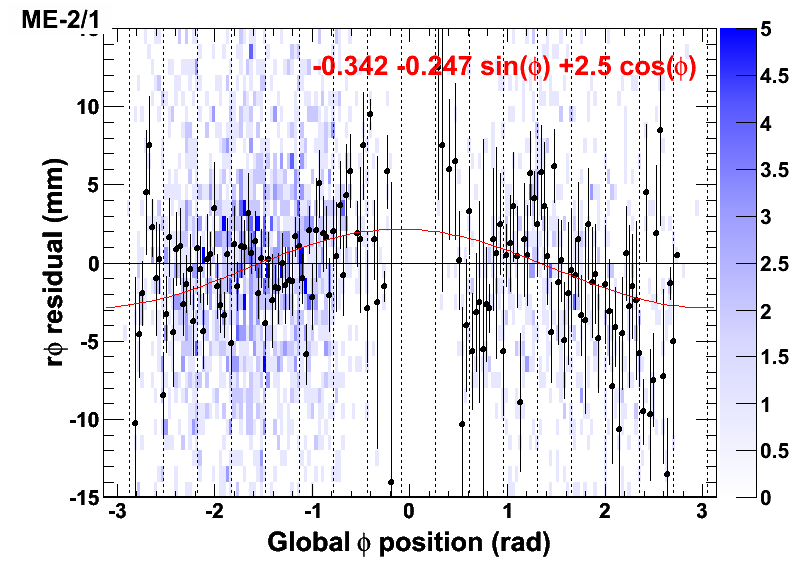
\includegraphics[width=0.5\linewidth]{cosmics_mem21.png}
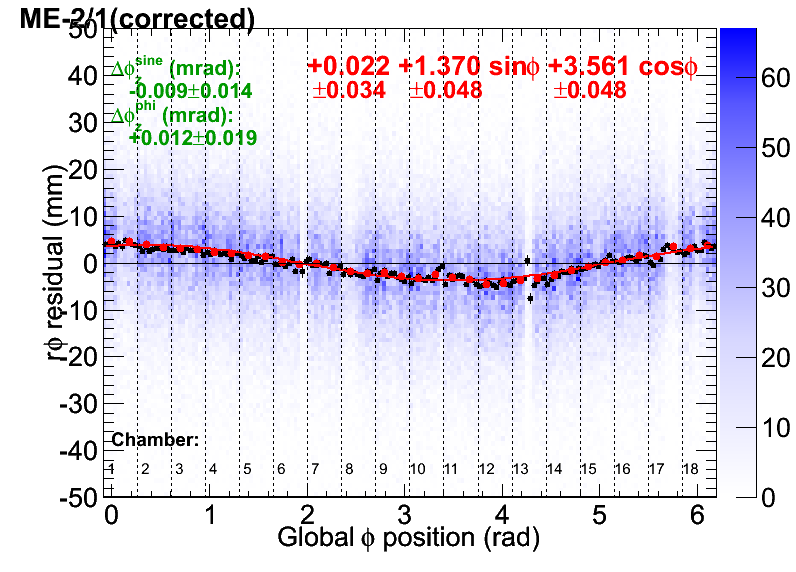
\includegraphics[width=0.5\linewidth]{one_and_only_mapplot.png}
\end{frame}

\begin{frame}
\frametitle{Magnetic field errors?}

\begin{itemize}
\item Observed charge asymmetry at high radius (distance from the beamline $\rho$); plot below is $r\phi$ residuals vs.\ $\rho$ for $\mu^+$ and $\mu^-$
\item Alignment is protected by residuals vs.\ $q/|p_z|$ fits
\item This splitting could be due to $\vec{B}$-field errors, material budget
\item Same pattern in all rings
\end{itemize}

\begin{center}
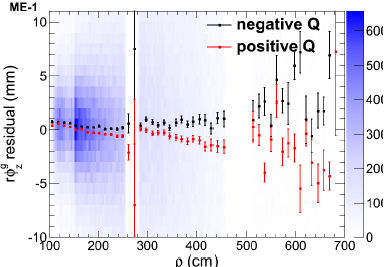
\includegraphics[width=0.7\linewidth]{rphi_plots_vs_rho_mem1.png}
\end{center}
\end{frame}

\begin{frame}
\frametitle{Systematics studies}

\begin{itemize}
\item Detailed systematic error studies quantifying the limits of
  interpretation of rings as a rigid body
\item Two studies shown below (left: variation vs.\ $\rho$, right:
  vs.\ $\phi$)
\end{itemize}

\vfill
\begin{columns}
\column{0.5\linewidth}
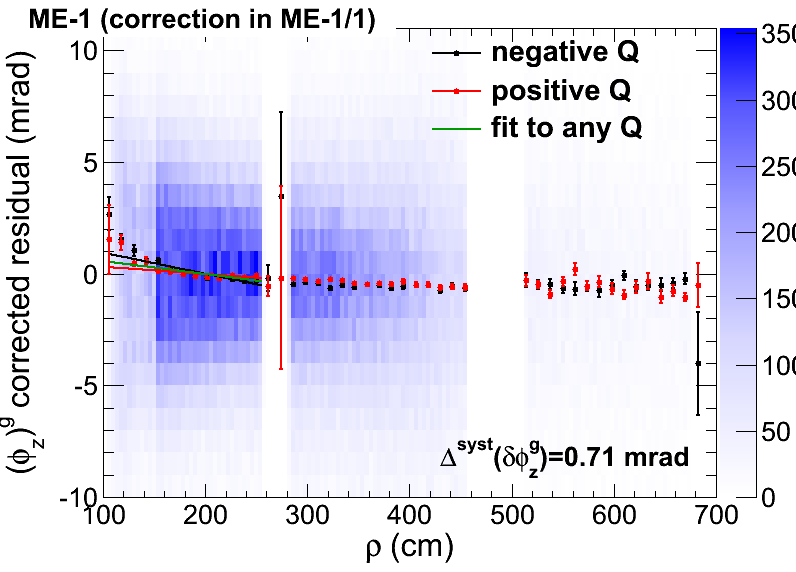
\includegraphics[width=\linewidth]{vsmomentum_correction.png}

\column{0.5\linewidth}
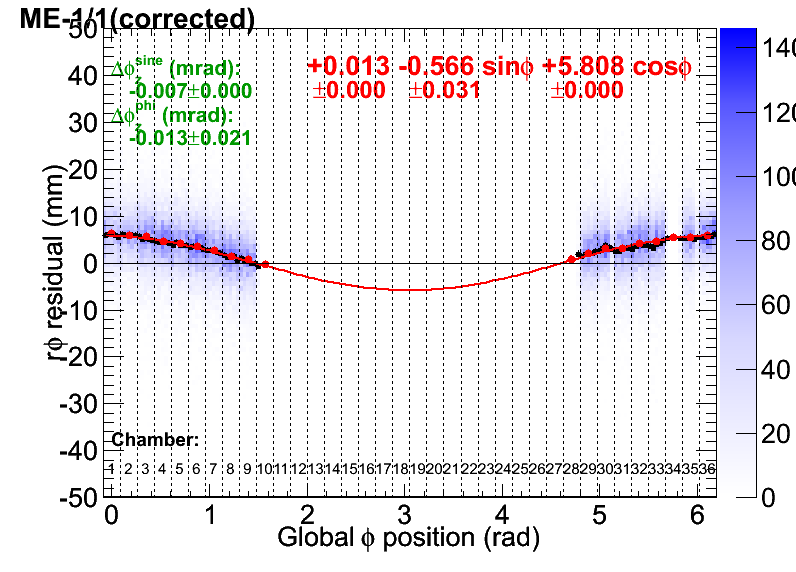
\includegraphics[width=0.5\linewidth]{vsphi_systematic1.png}
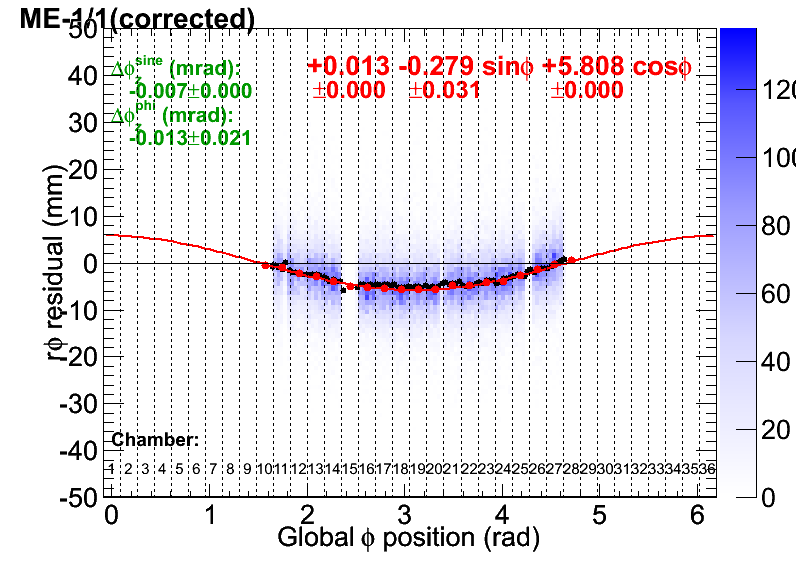
\includegraphics[width=0.5\linewidth]{vsphi_systematic2.png}

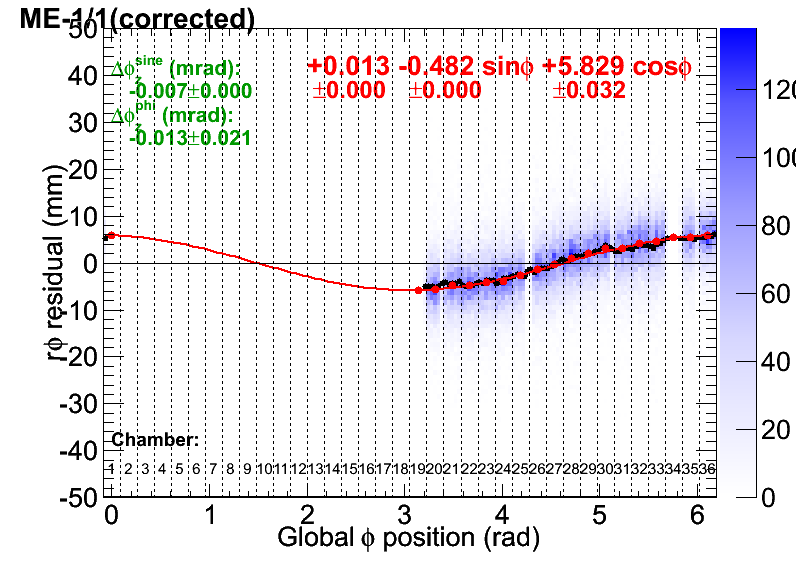
\includegraphics[width=0.5\linewidth]{vsphi_systematic3.png}
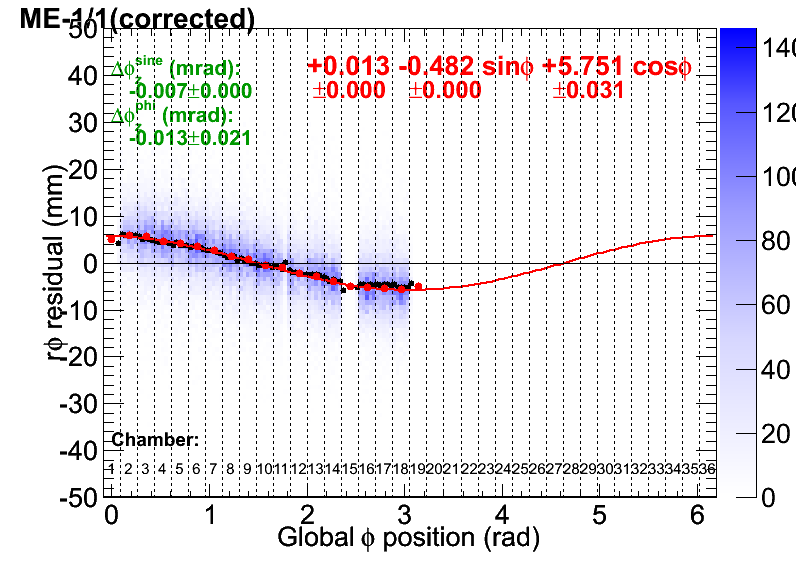
\includegraphics[width=0.5\linewidth]{vsphi_systematic4.png}
\end{columns}
\end{frame}

\begin{frame}
\frametitle{Residuals-calculation method}

\begin{itemize}
\item Statistical and systematic uncertainties
\item Comparison of results for different methods of residuals calculation
\begin{itemize}
\item this distinction between ``TrackerMuons'' and ``GlobalMuons''
  are what Aysen is studying, but while it has noticible effects
  inside of individual chambers in the barrel, it has less of an
  effect when finding the average position of a ring
\end{itemize}
\end{itemize}

\vfill
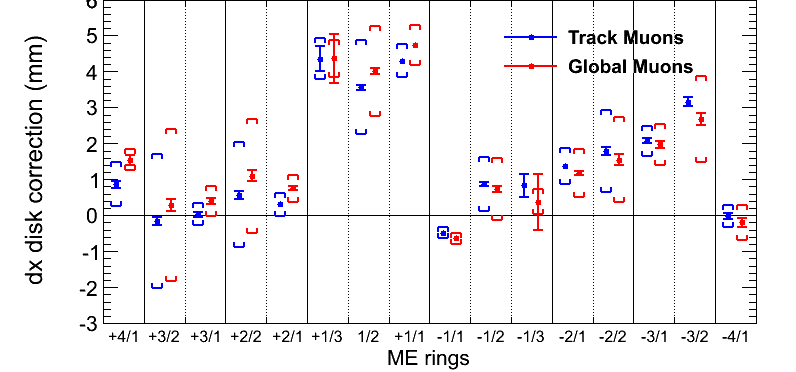
\includegraphics[width=\linewidth]{finaltkgb1.png}
\end{frame}

\begin{frame}
\frametitle{Independent cross-check}

\begin{columns}
\column{0.67\linewidth}
\begin{columns}
\column{0.5\linewidth}
\centering Before alignment

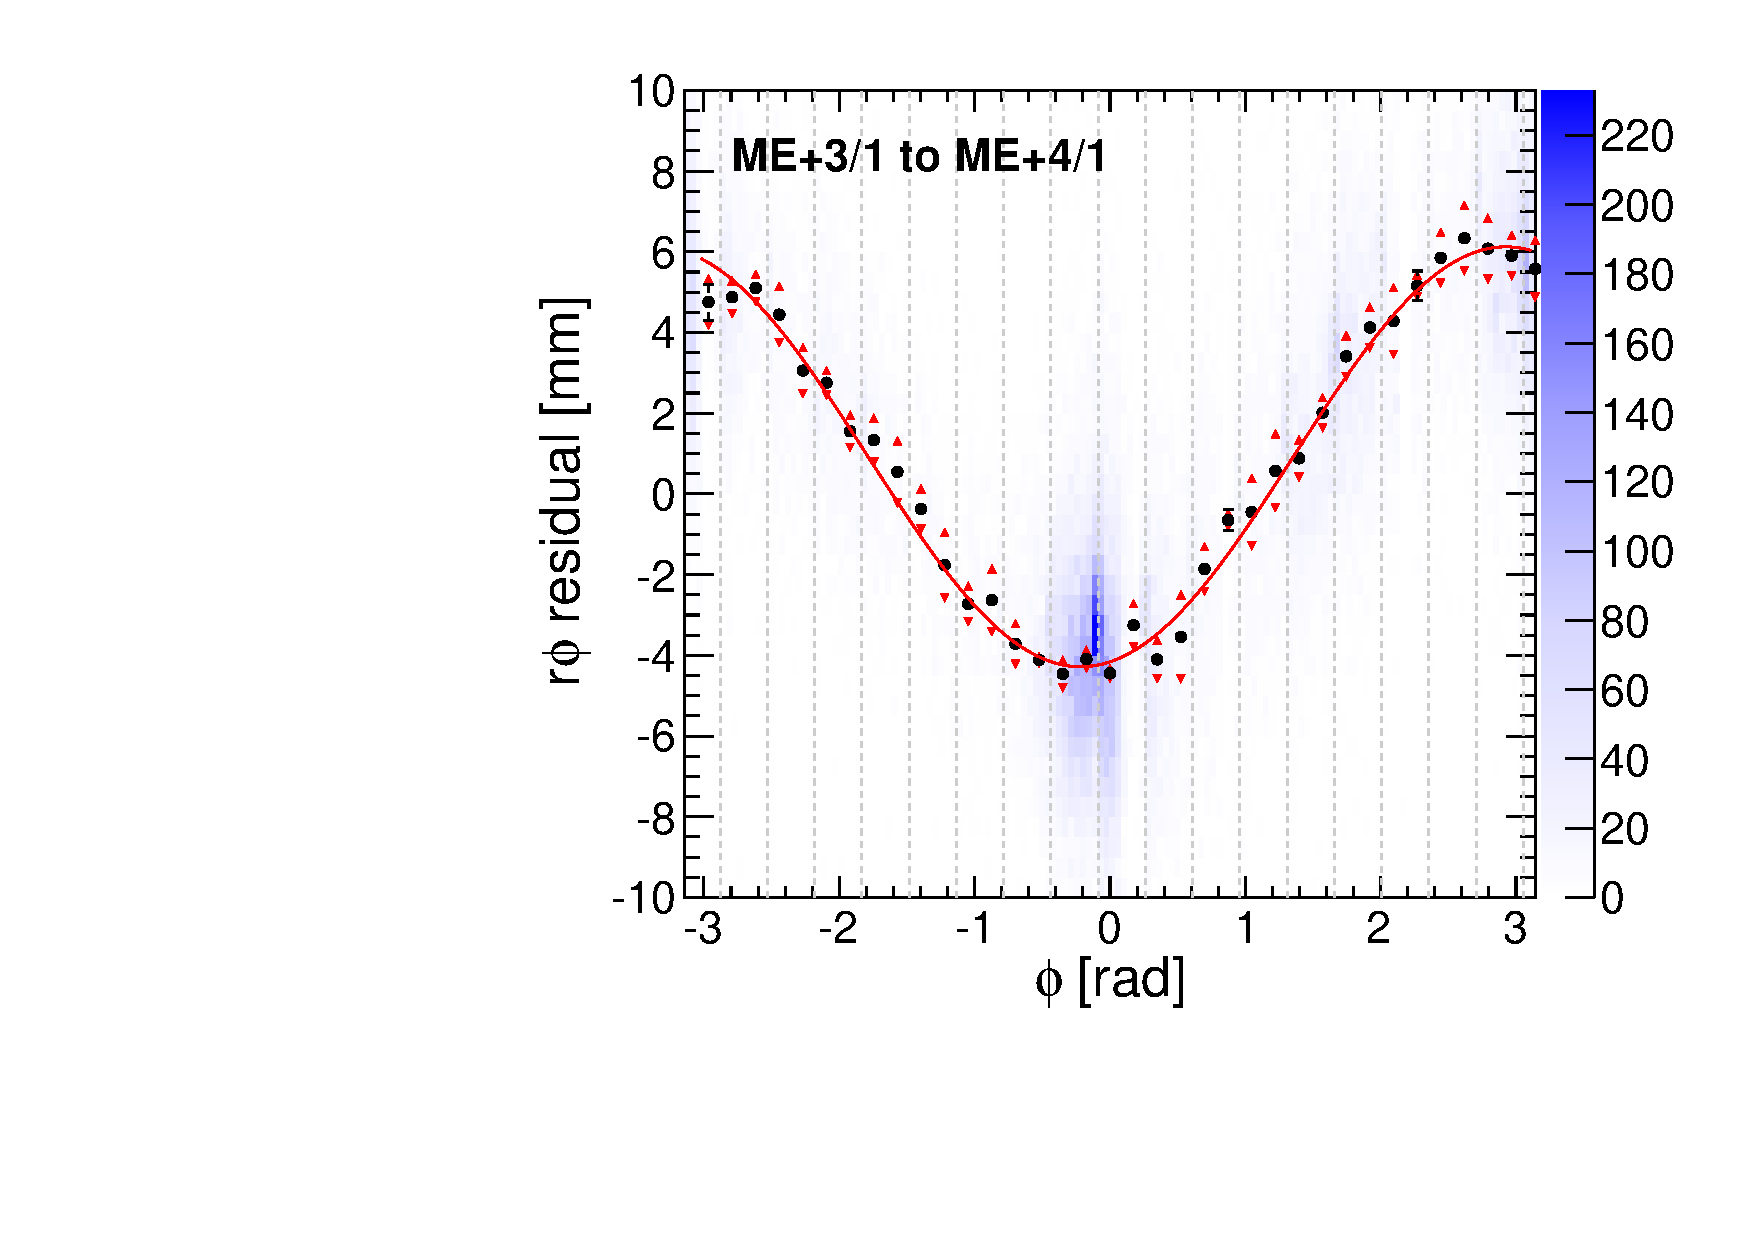
\includegraphics[width=\linewidth]{BHCrossCheck_mep41_before.pdf}

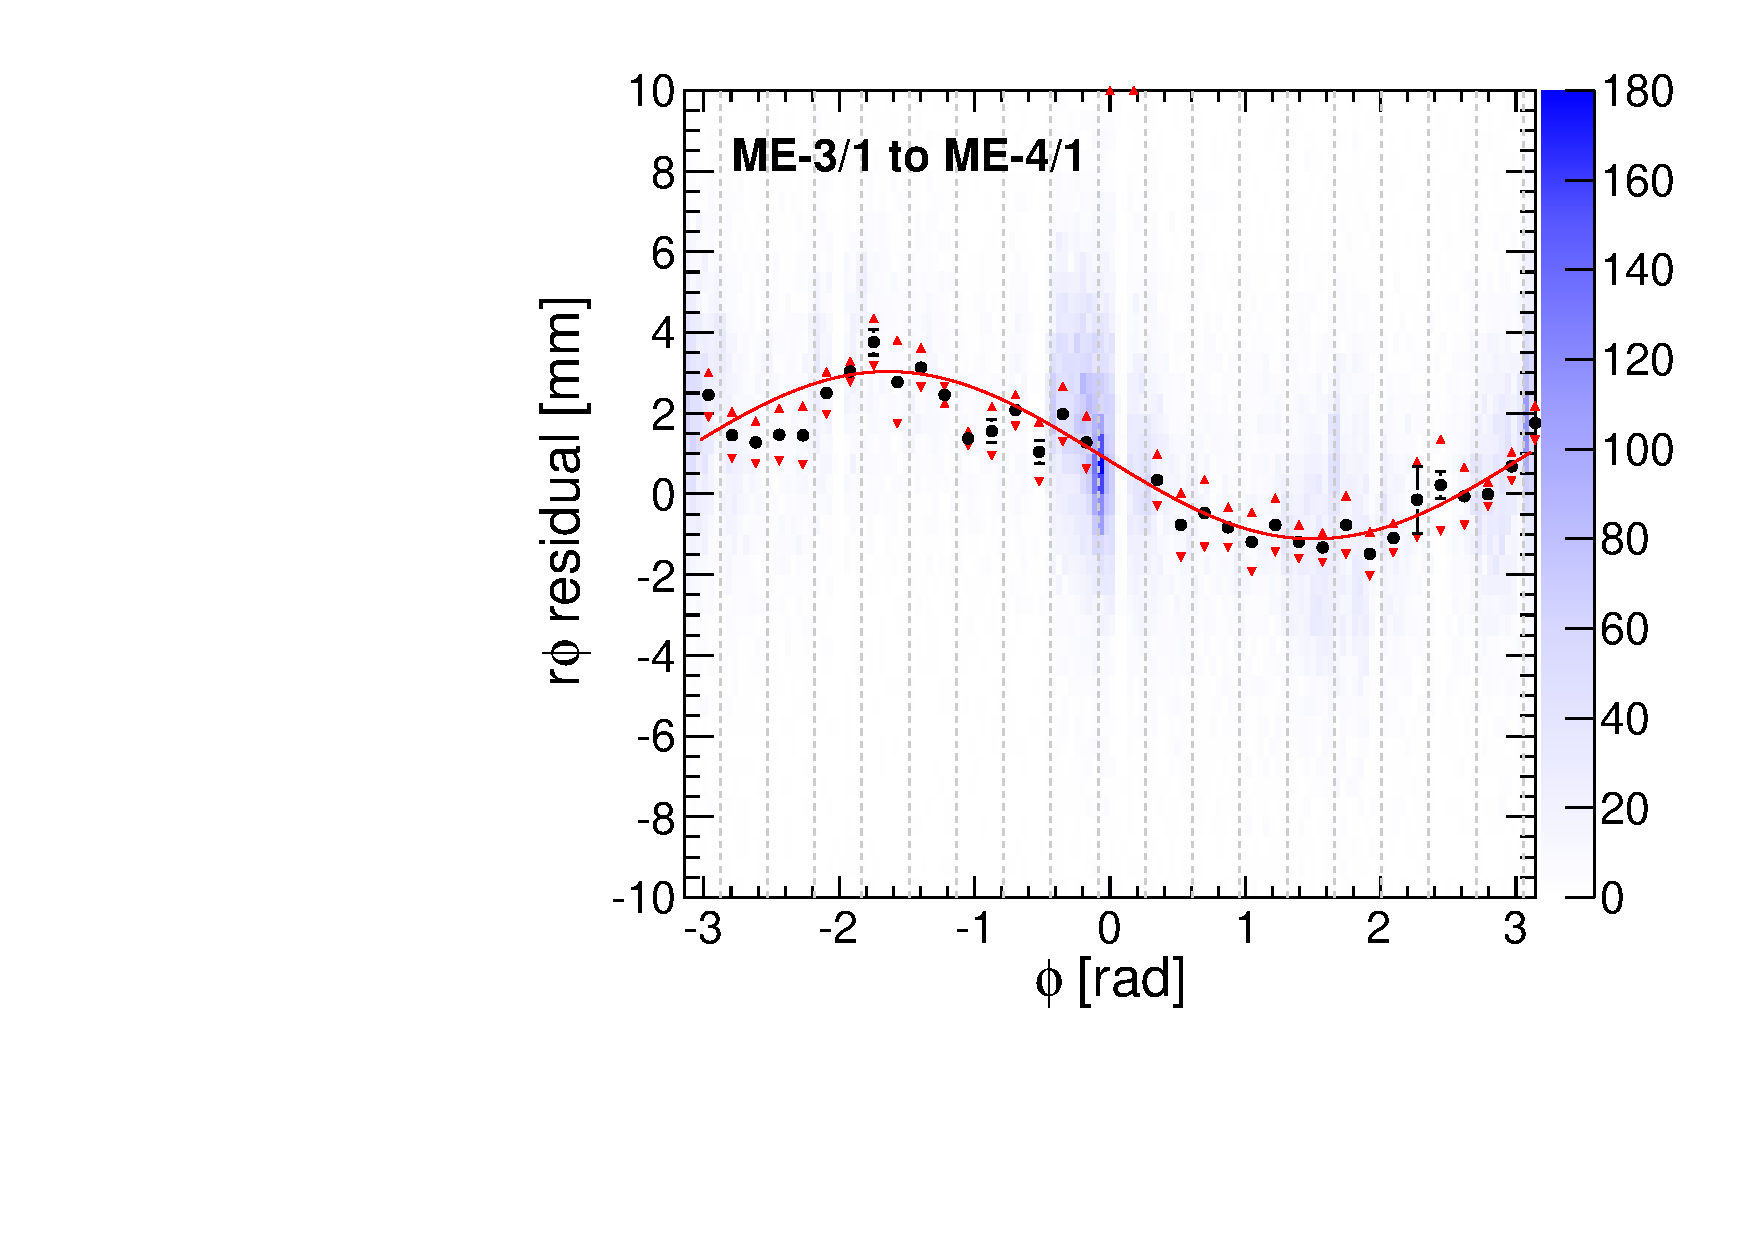
\includegraphics[width=\linewidth]{BHCrossCheck_mem41_before.pdf}

\column{0.5\linewidth}
\centering After alignment

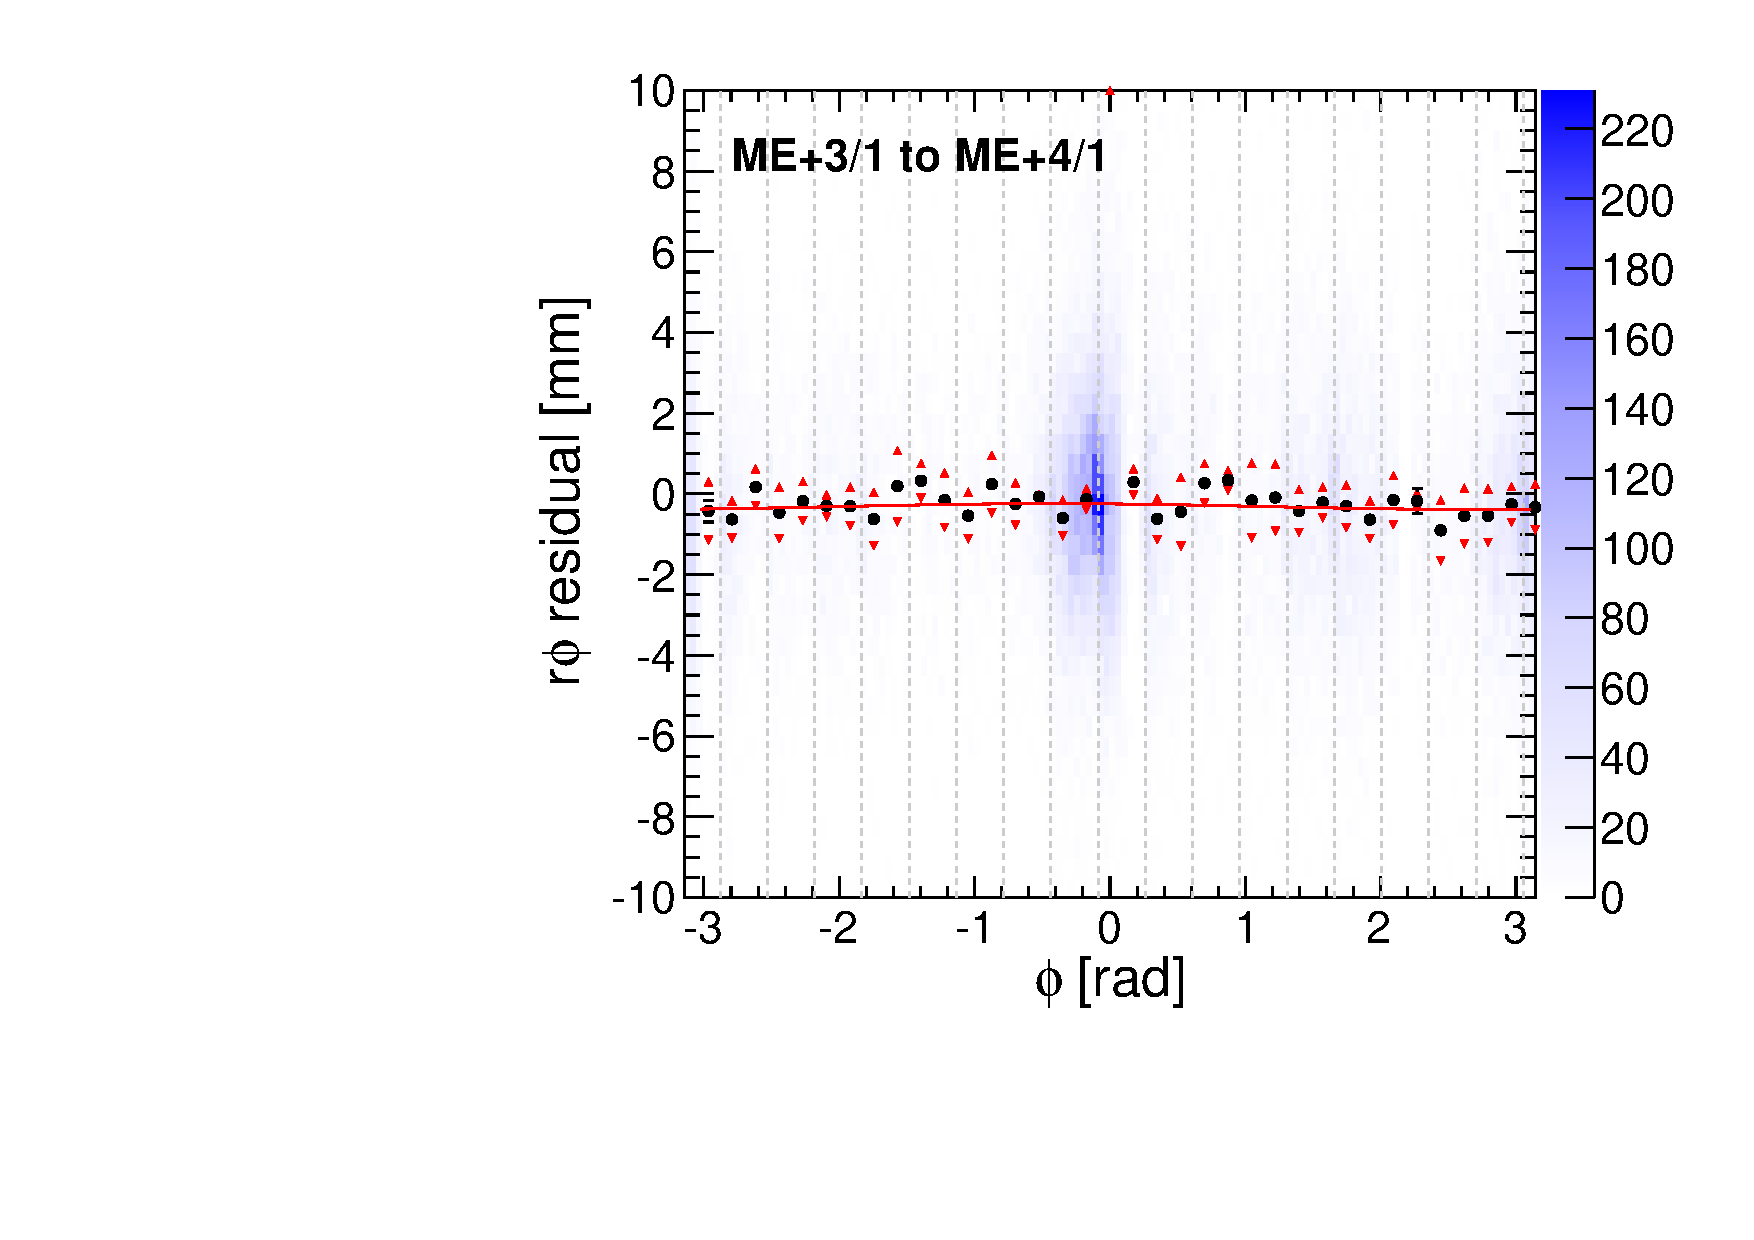
\includegraphics[width=\linewidth]{BHCrossCheck_mep41_after.pdf}

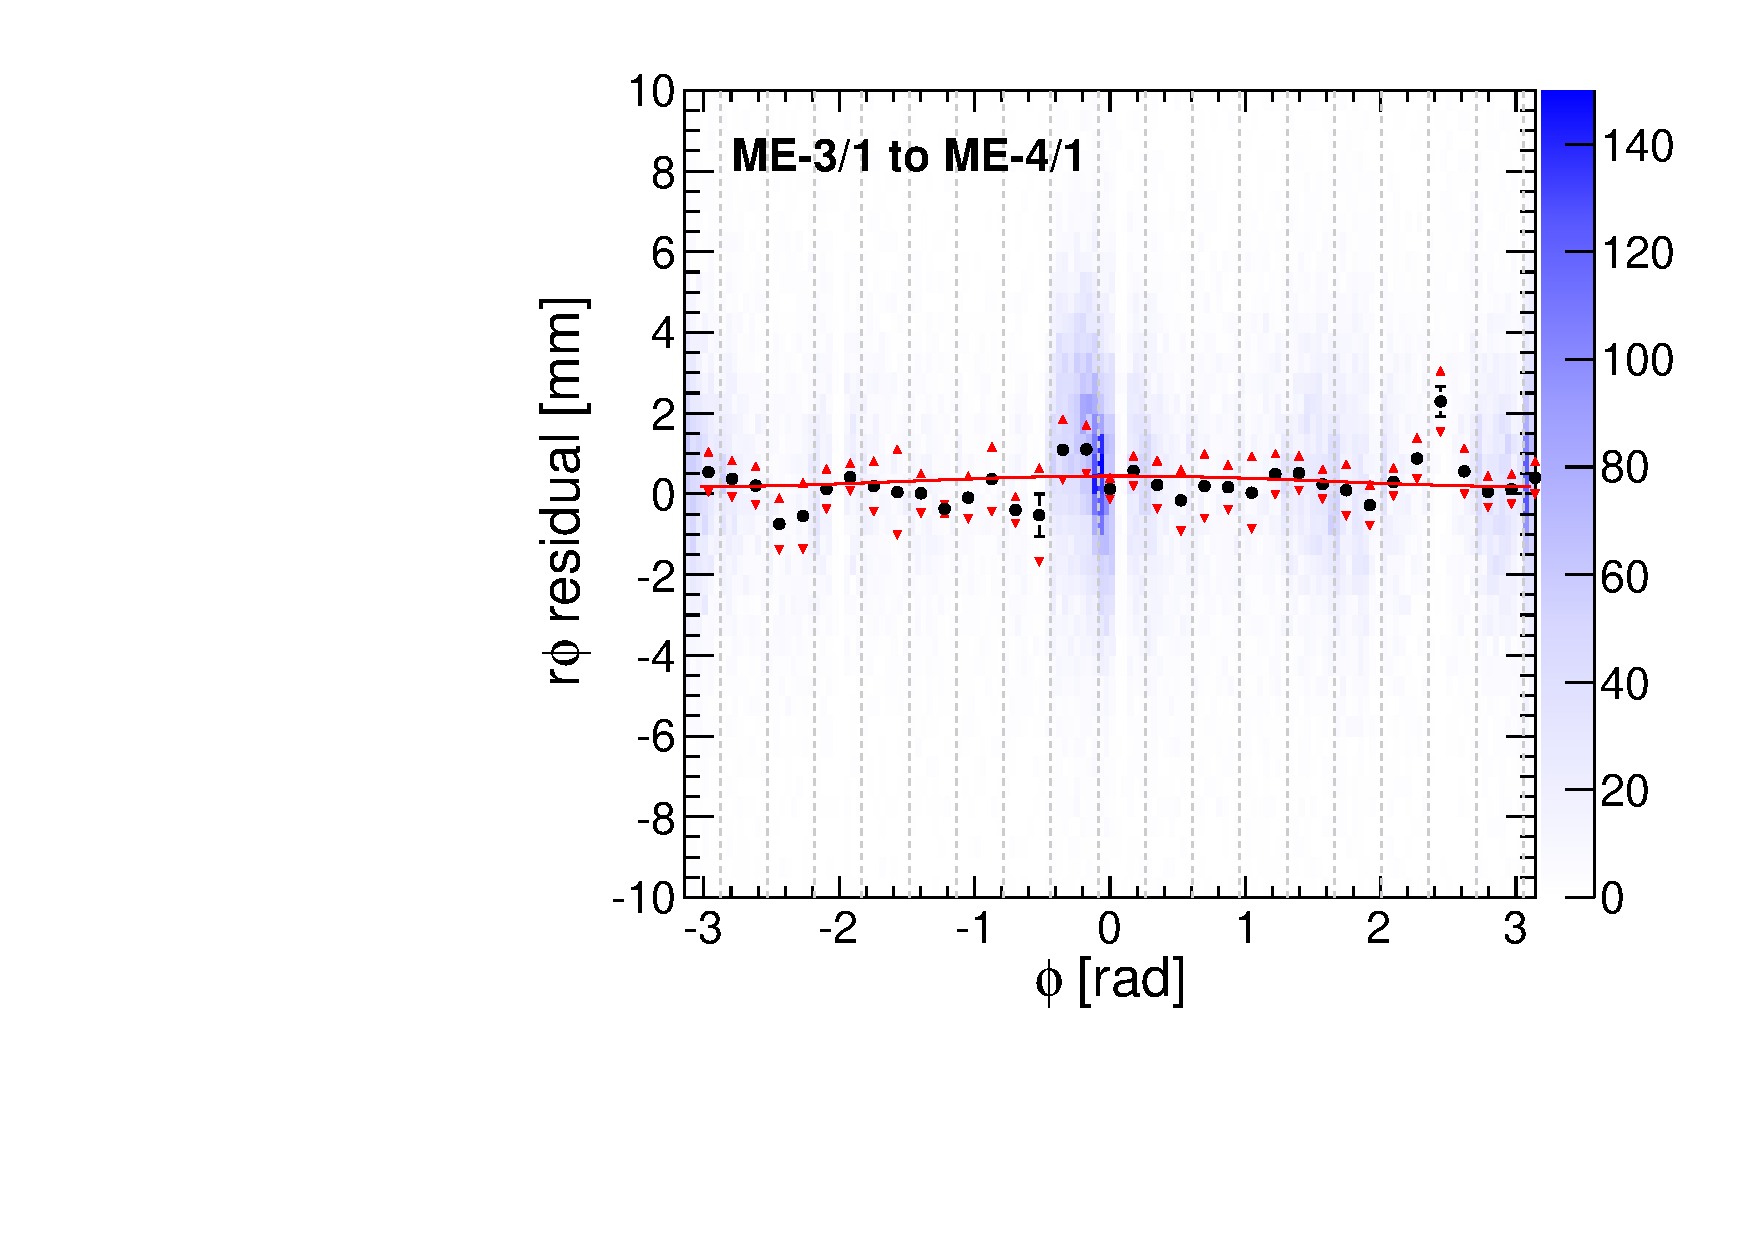
\includegraphics[width=\linewidth]{BHCrossCheck_mem41_after.pdf}
\end{columns}

\vspace{0.3 cm}
\centering \textcolor{darkblue}{The above plots were not used for the alignment--- they are a cross-check}

\column{0.33\linewidth}
\begin{itemize}
\item Ring alignment relative to the tracker verified with ring
  alignment relative to other rings using beam-halo tracks (note $\phi$ asymmetry)

\item Independent alignment techniques yield the same result within
  130~$\mu$m ($x$ and $y$) and 0.14~mrad ($\phi_z$) for ME4/1
\end{itemize}
\end{columns}
\end{frame}

\begin{frame}
\frametitle{Do internal alignments factorize?}

\begin{itemize}
\item Reproducibility of internal ring alignment after the whole ring
  has been re-positioned depends on pattern of photogrammetry constraints
\item ME$\pm$1/2 each have two antipodal constraints which pull the
  ring back toward the photogrammetry's coordinate frame
\item The rest of the rings are fine
\end{itemize}

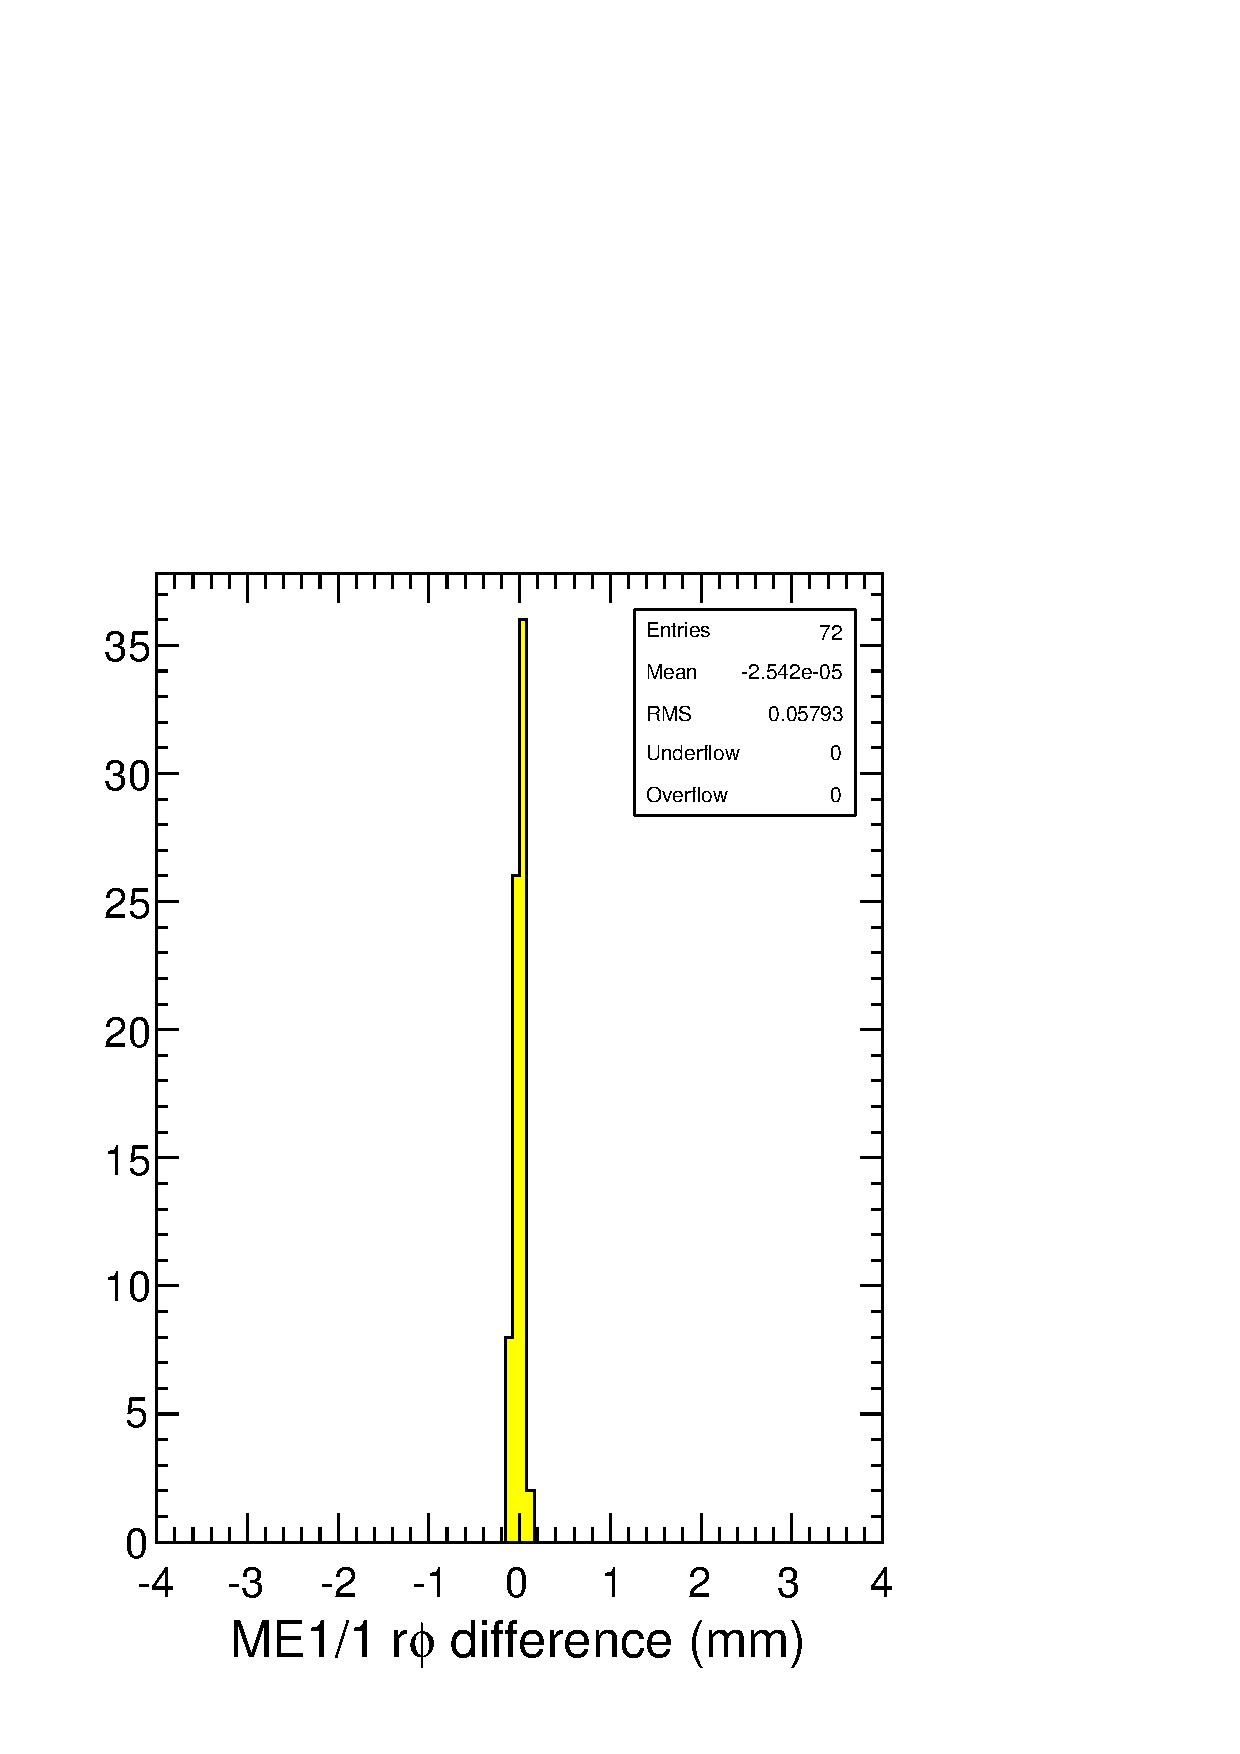
\includegraphics[width=0.24\linewidth]{effectofdisk_me11.pdf}
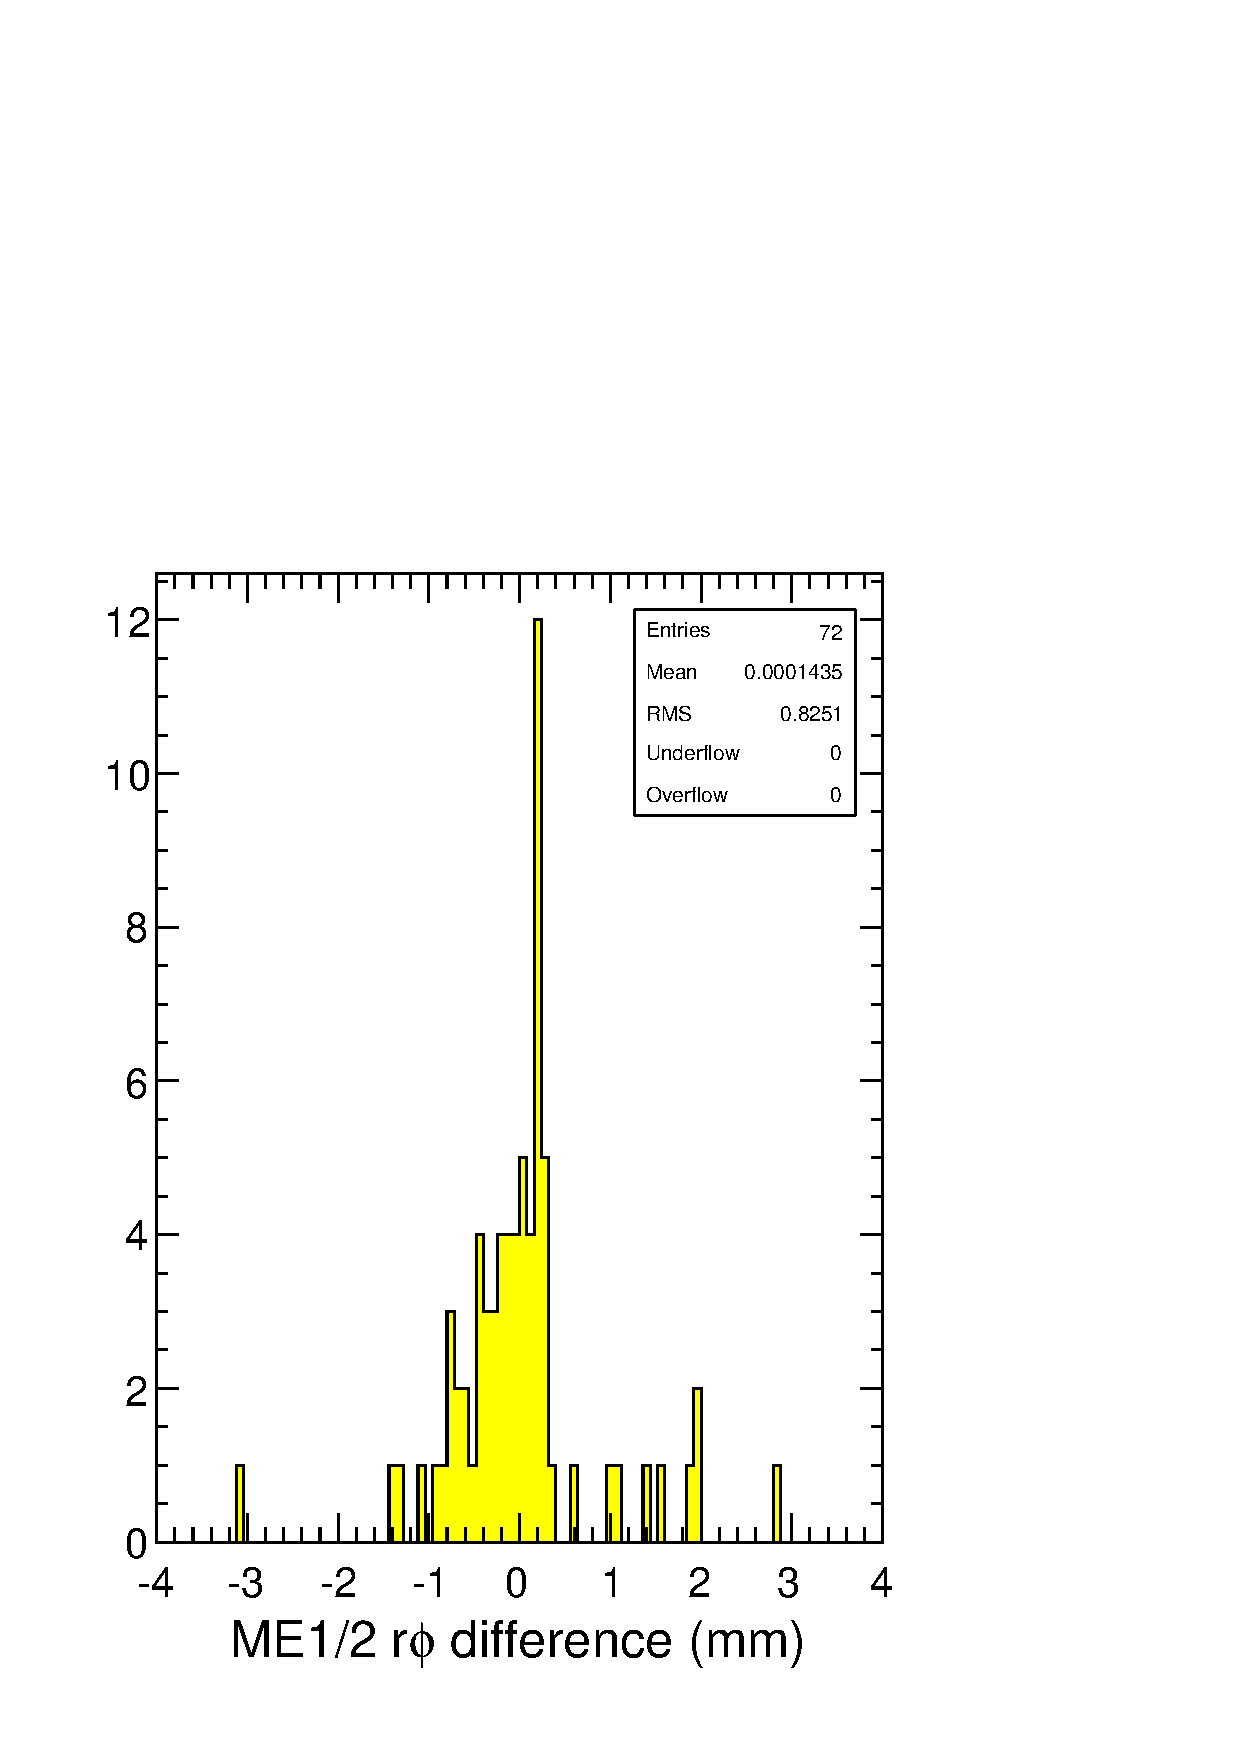
\includegraphics[width=0.24\linewidth]{effectofdisk_me12.pdf}
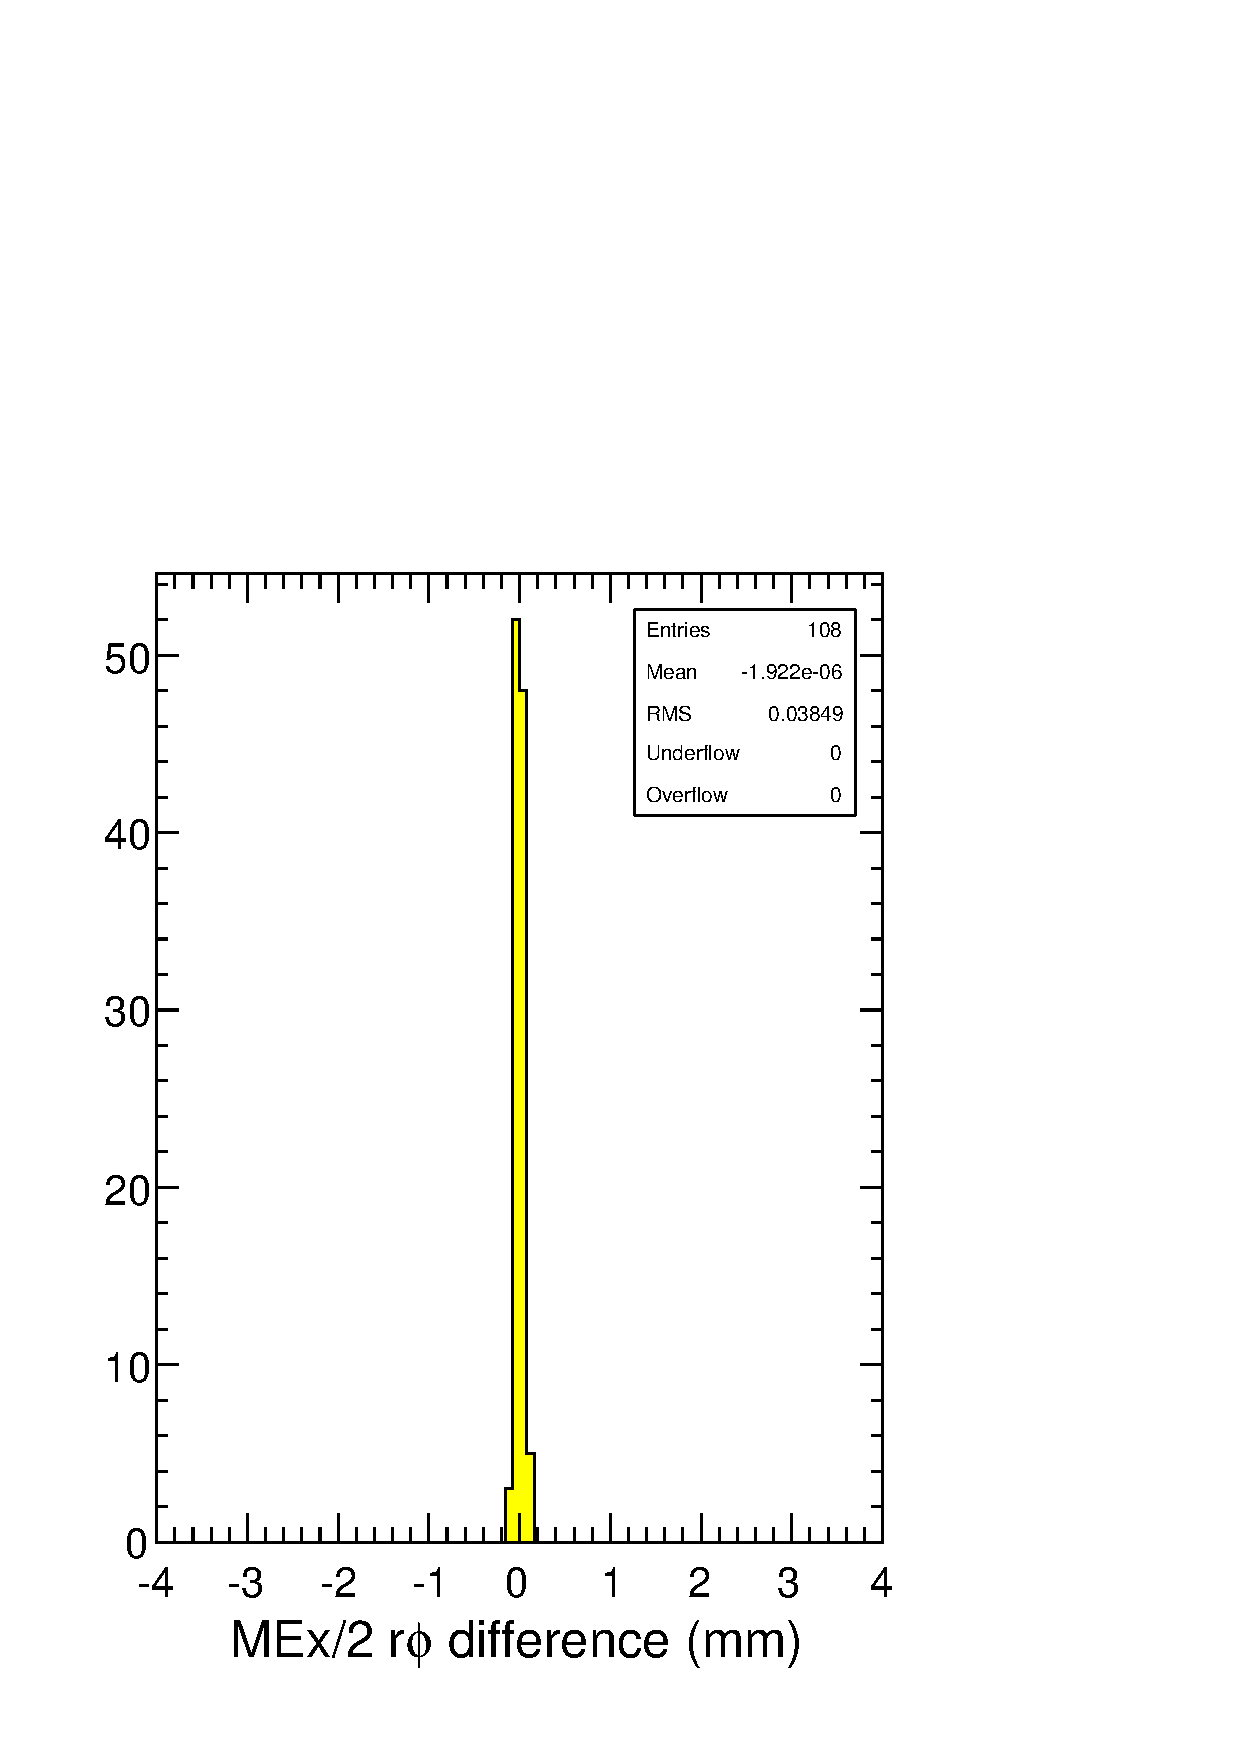
\includegraphics[width=0.24\linewidth]{effectofdisk_inner234.pdf}
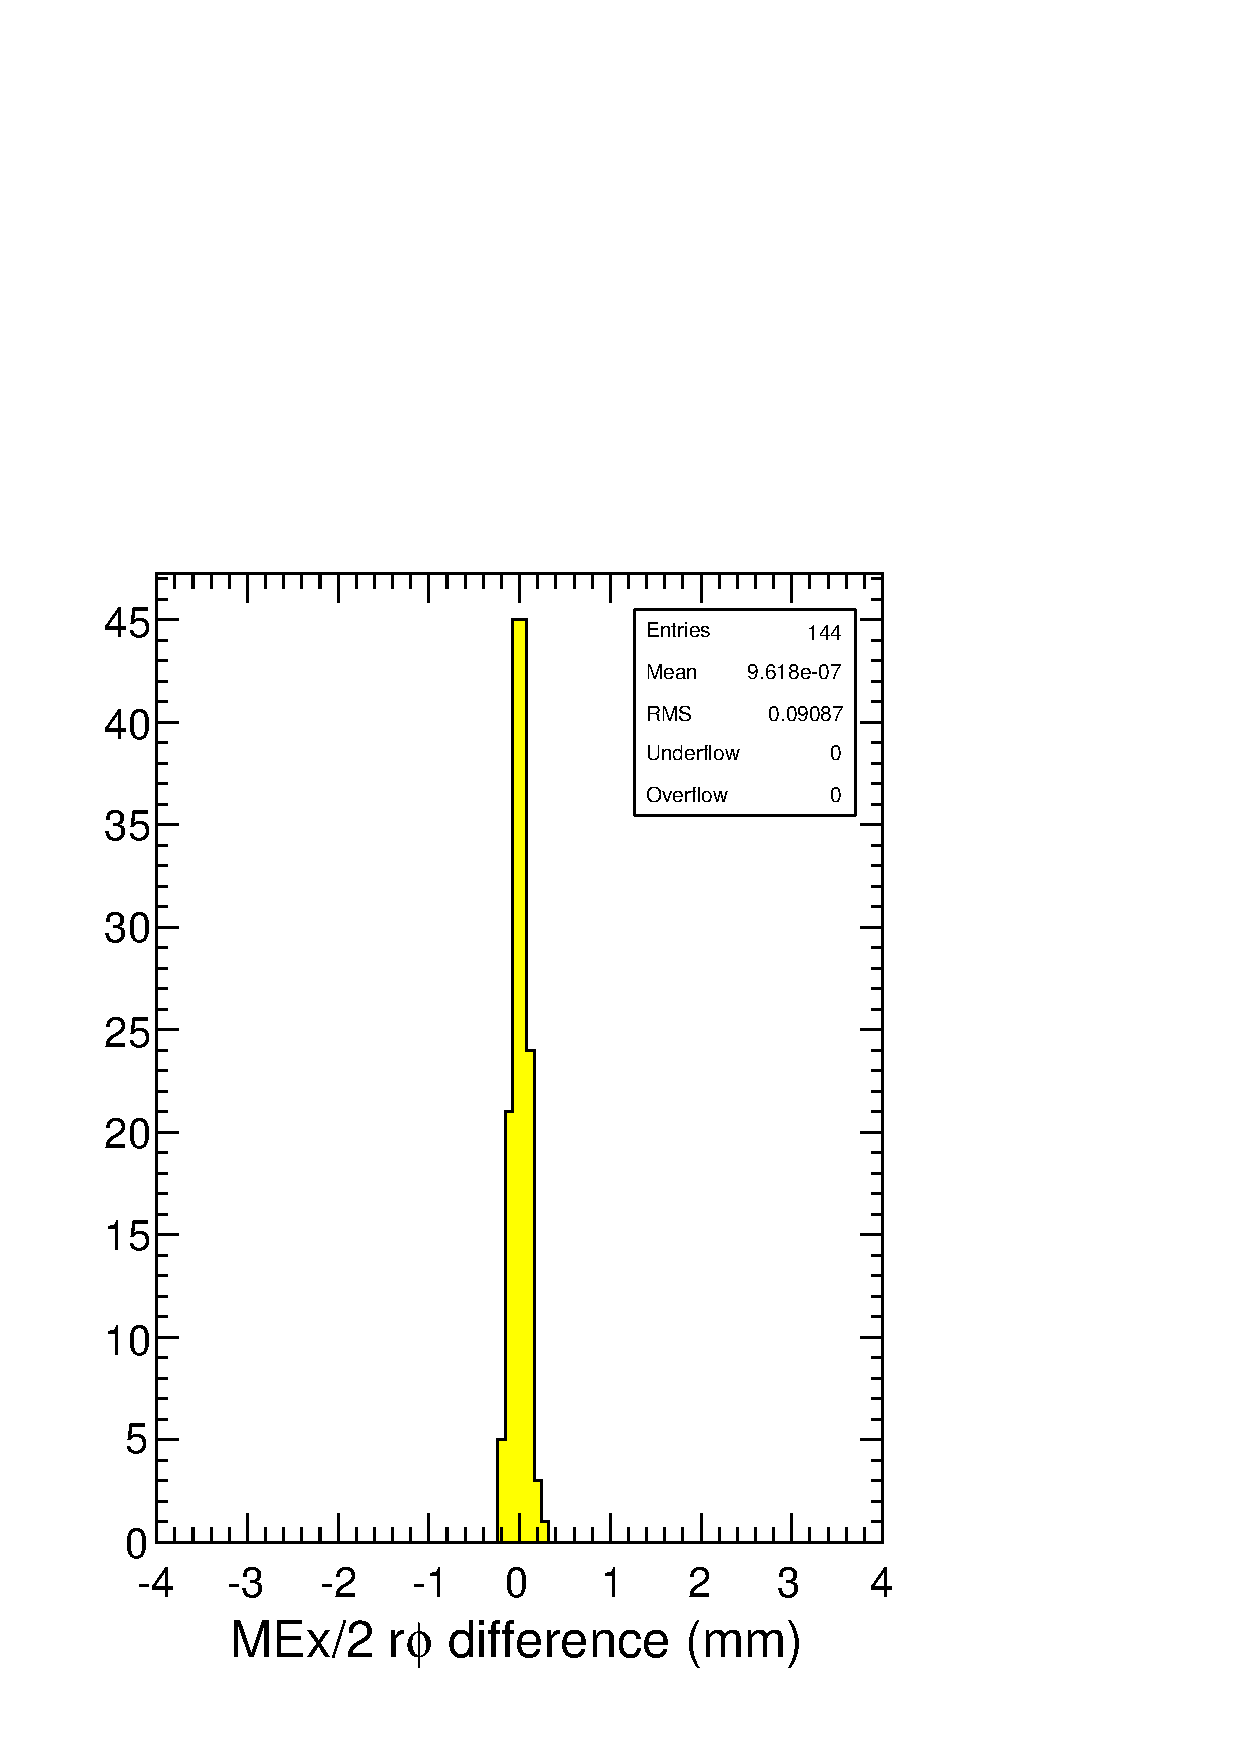
\includegraphics[width=0.24\linewidth]{effectofdisk_outer.pdf}
\end{frame}

\begin{frame}
\frametitle{Change in internal alignment}

\begin{itemize}
\item To solve this problem, never use more than one photogrammetry constraint per ring

\item \textcolor{darkblue}{Before} (this is the ``spread'' in ME$\pm$1/2 chamber positions):

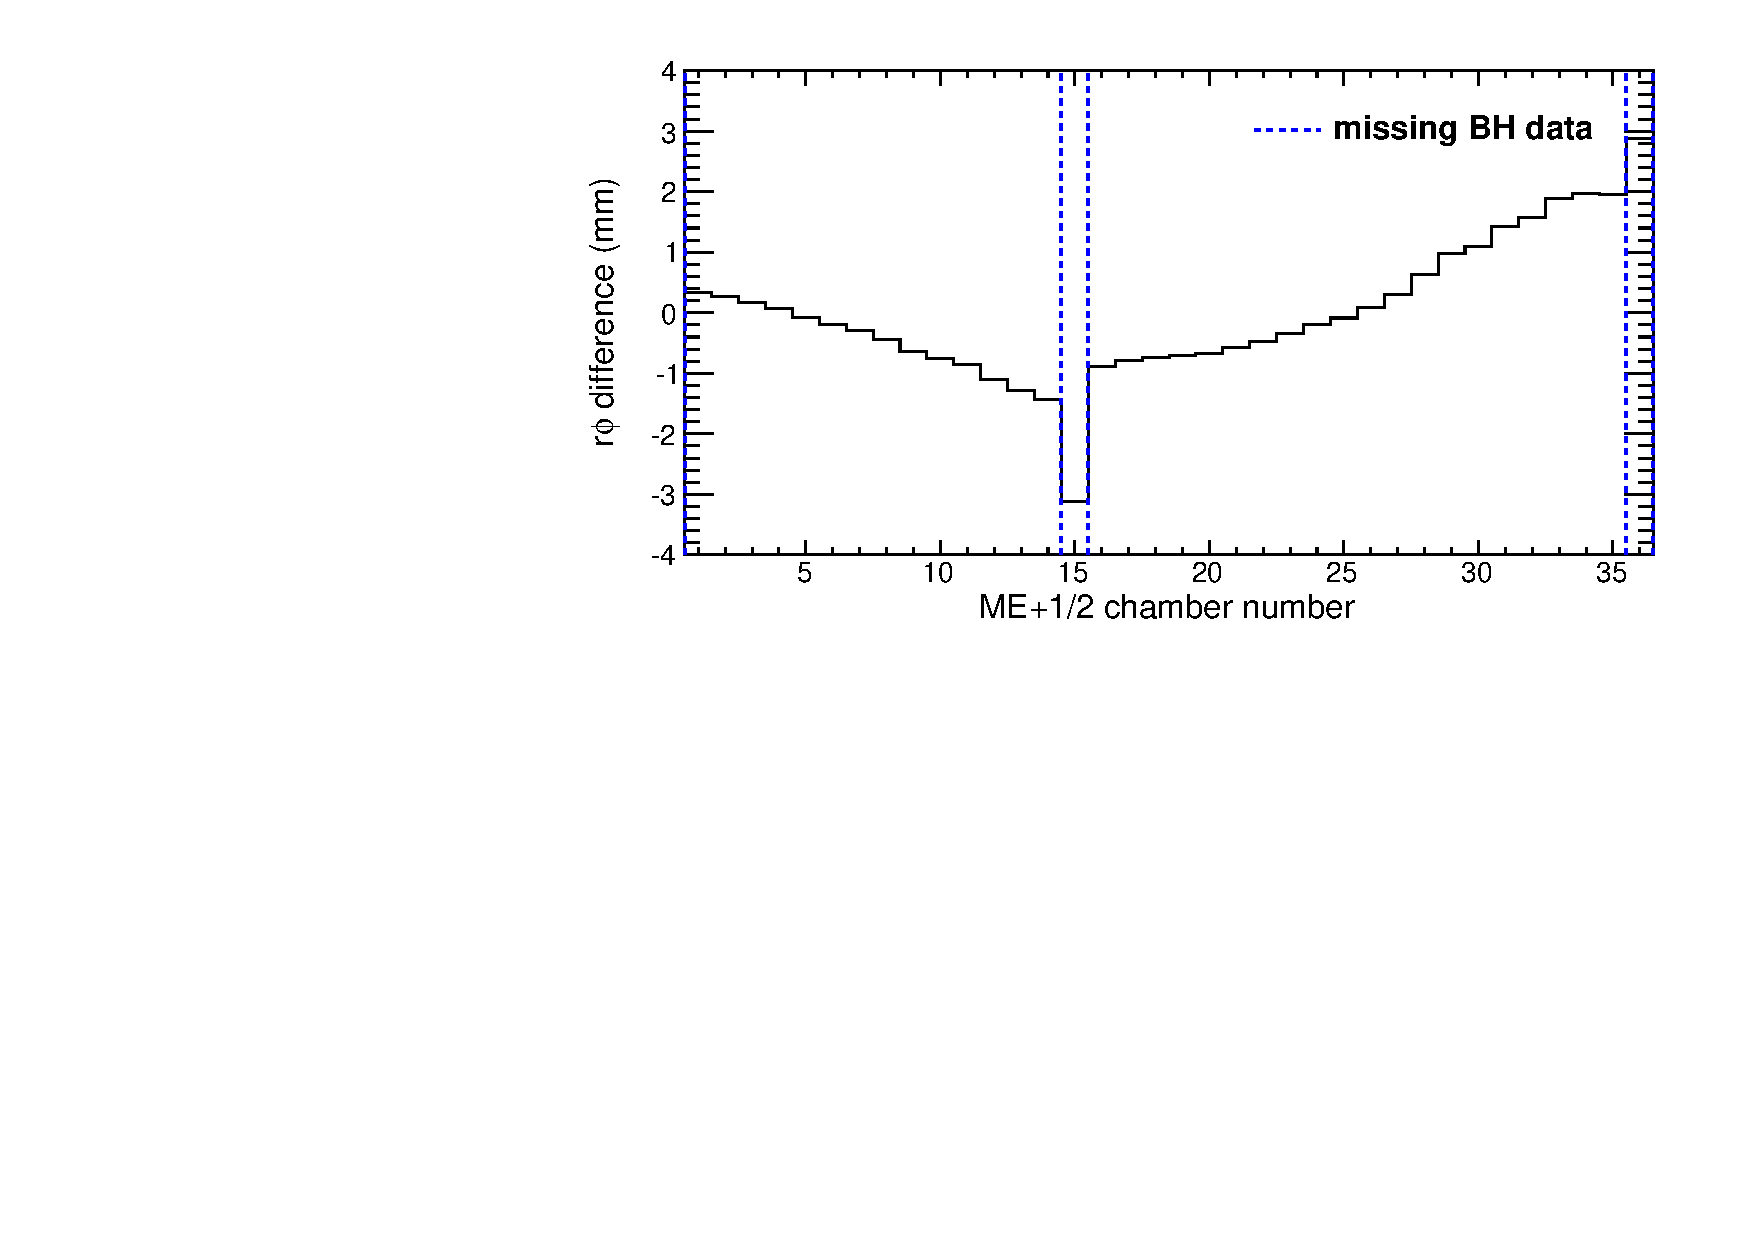
\includegraphics[width=0.5\linewidth]{effectofdisk_ring_mep12.pdf}
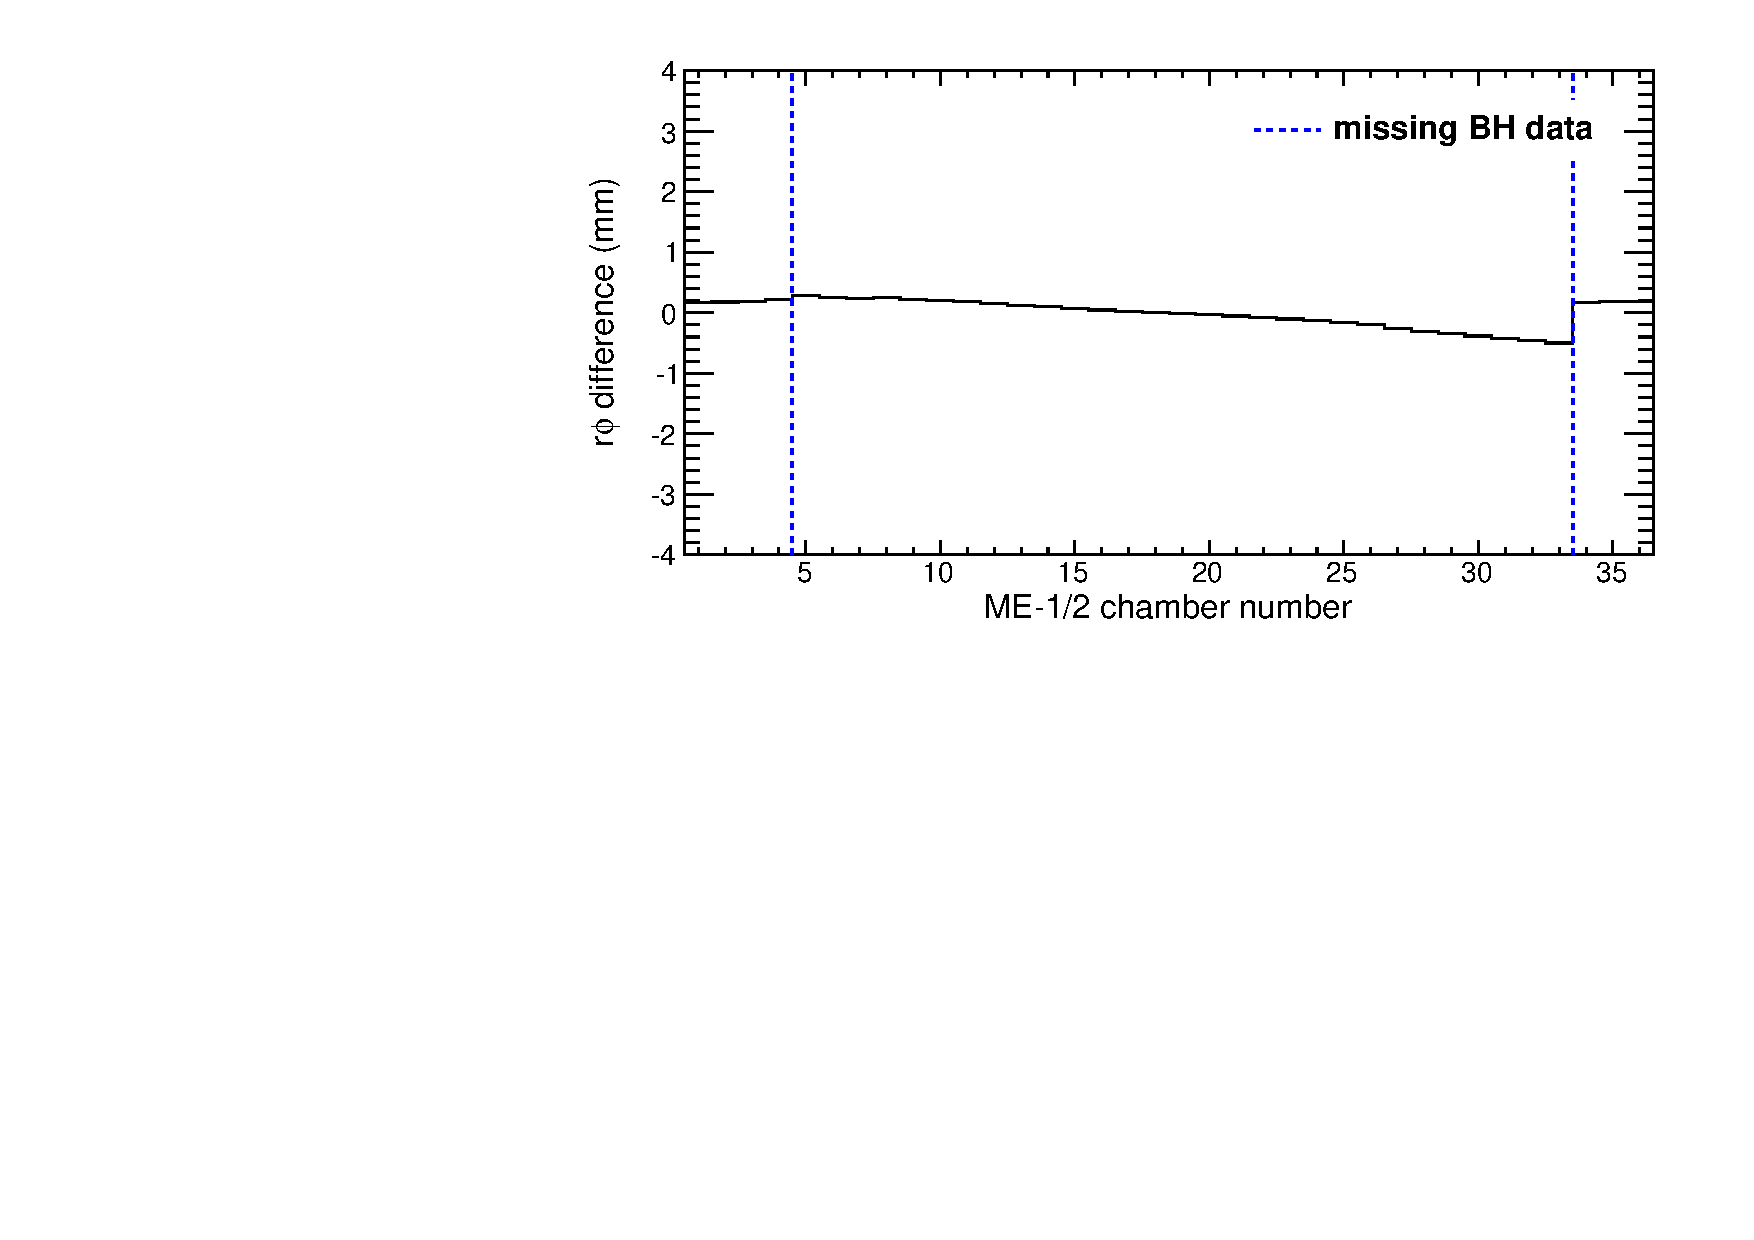
\includegraphics[width=0.5\linewidth]{effectofdisk_ring_mem12.pdf}

\item \textcolor{darkblue}{After:} PG only constrains the relative positions of ME$+$1/2/15
  (and neighbors) and ME$-$1/2/33,34

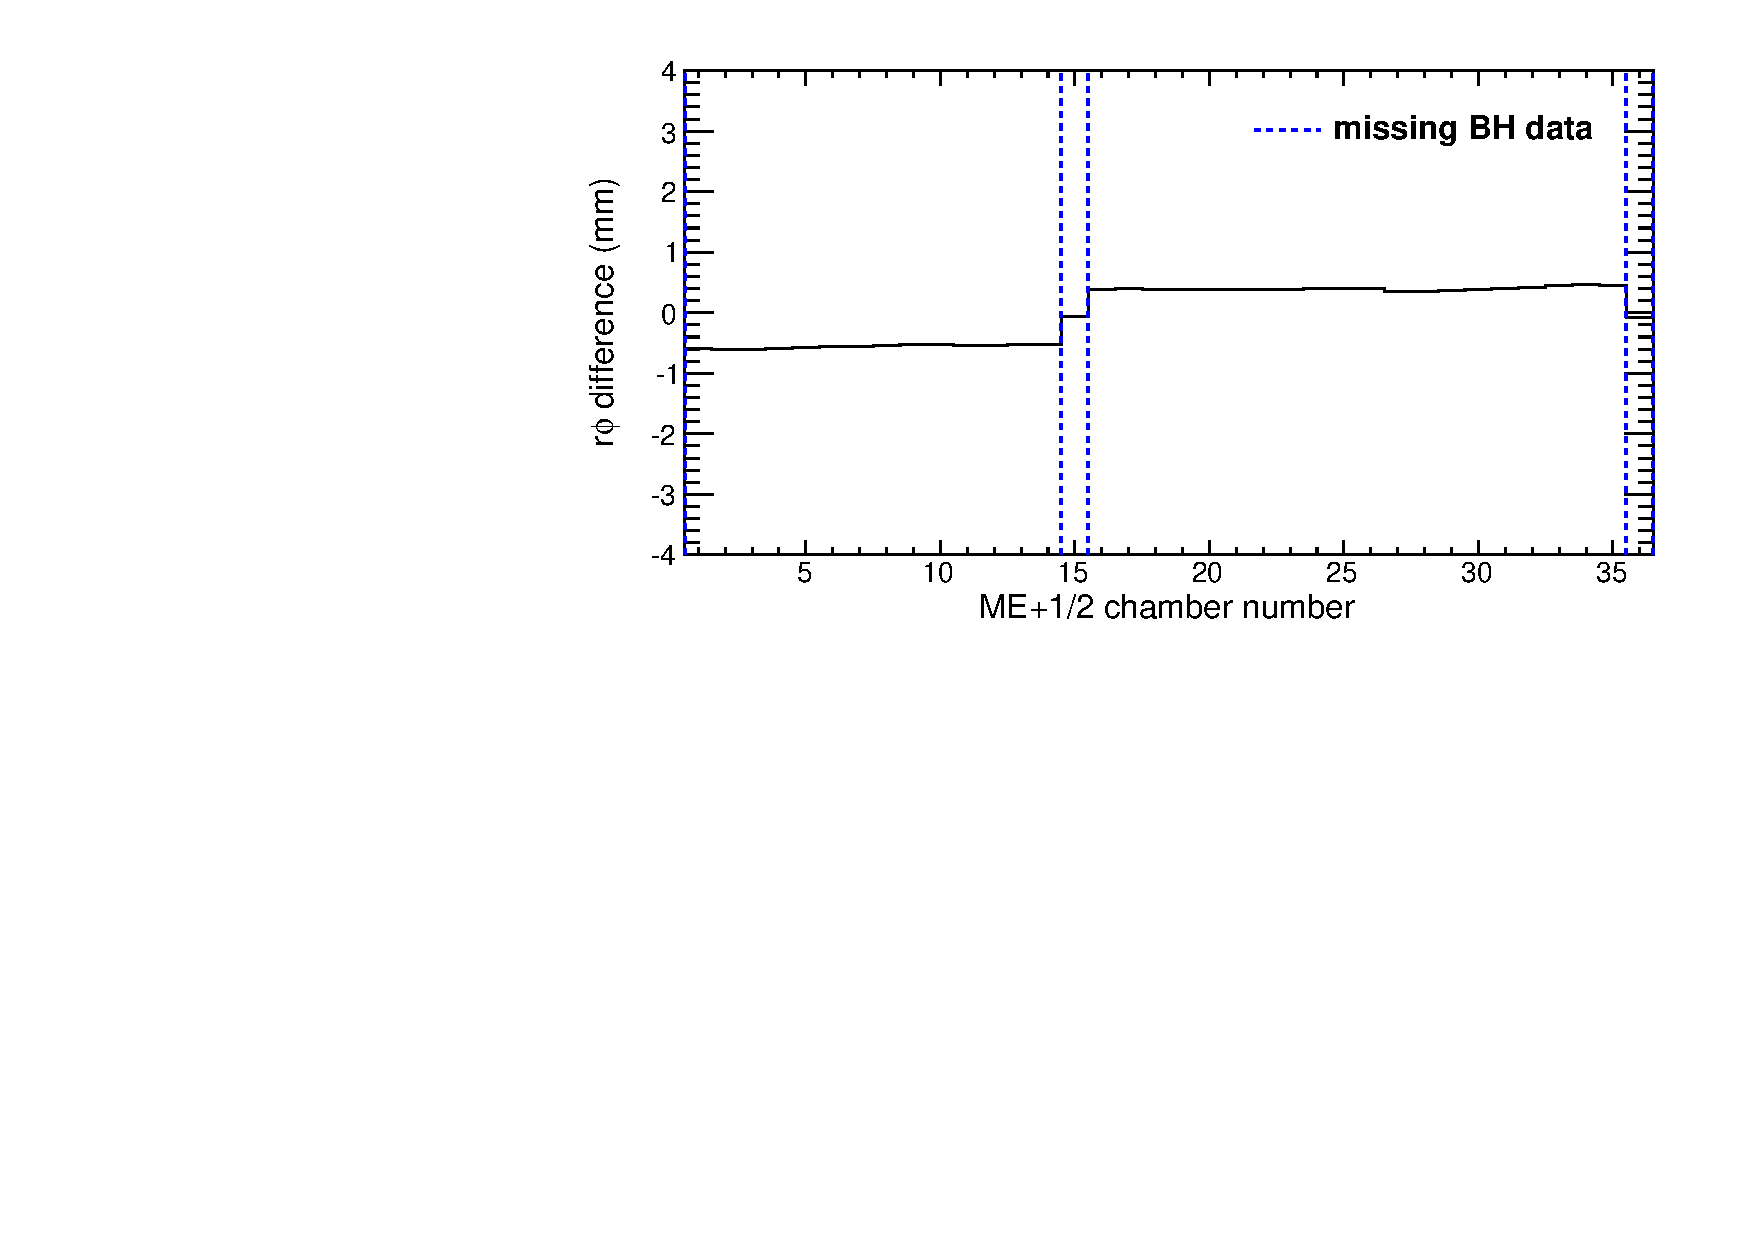
\includegraphics[width=0.5\linewidth]{effectofdiskOnlyOne_ring_mep12.pdf}
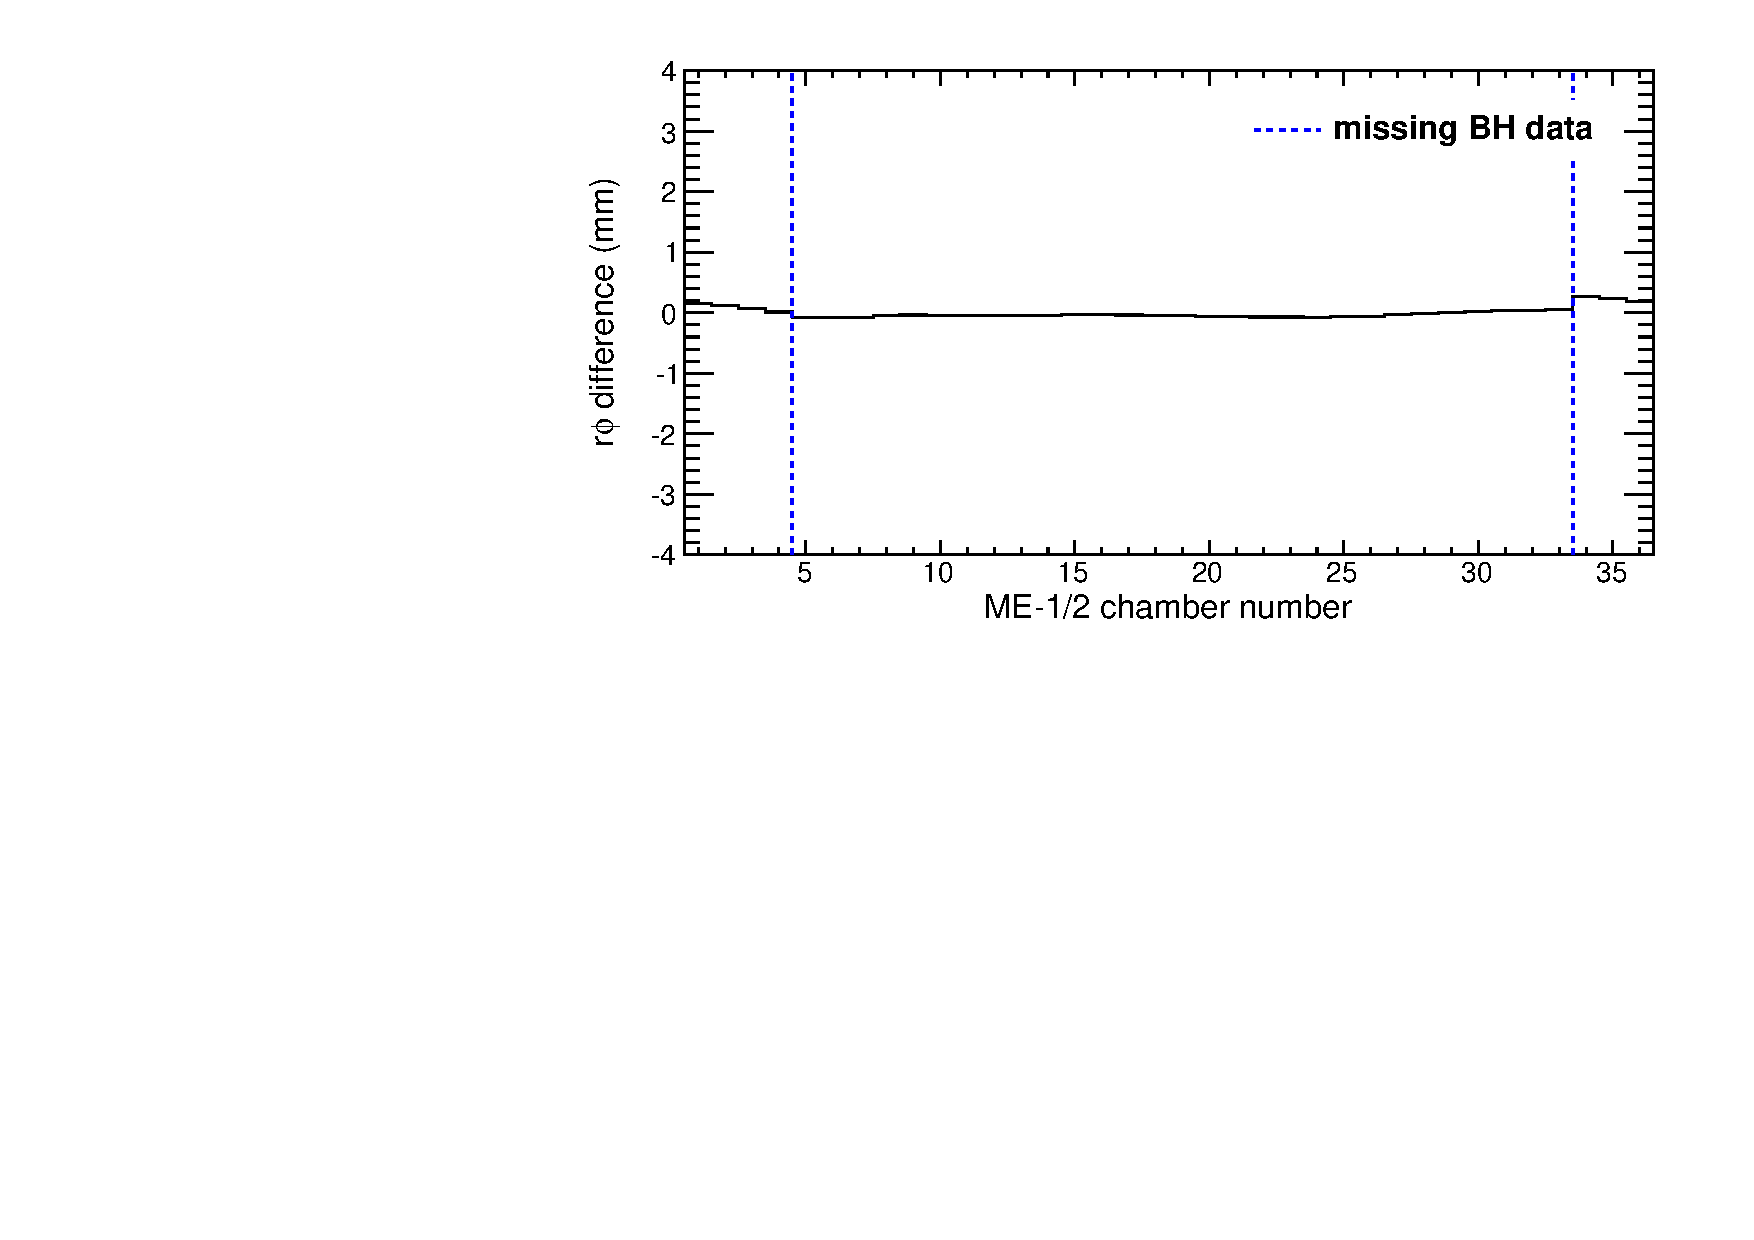
\includegraphics[width=0.5\linewidth]{effectofdiskOnlyOne_ring_mem12.pdf}
\end{itemize}
\end{frame}

%% \section*{First section}
%% \begin{frame}
%% \begin{center}
%% \Huge \textcolor{blue}{First section}
%% \end{center}
%% \end{frame}

\begin{frame}
\frametitle{For full details}

\textcolor{darkblue}{\Large see the ``Endcap ring alignment note'' on Indico}

\vfill
\hspace{-0.83 cm} \textcolor{darkblue}{\Large Next steps}

\vspace{0.2 cm}
\begin{enumerate}
\item Proposing new internal ring constants for sign-off
\item Proposing ring alignment relative to tracker method for sign-off
\item Must repeat ring alignment relative to tracker with the updated
  tracker description and cross-alignment before Nov.~12
\item Will likely finish much, much sooner because all of the pieces
  are already in place
\item When those constants are signed-off (via HyperNews), they need
  to be uploaded to the database and the Muon POG should be pointed to
  their location and how to use them
\end{enumerate}
\label{numpages}
\end{frame}

\end{document}
